\section{Introducción}

En la hidrodinámica se observa un fenómeno denominado como el \textit{equilibrio
hidrostático}. Un fluido que está en equilibrio hidrostático está sometido a un
balance de fuerzas: aquellas que actúan en la dirección interna al fluido, y
aquellas causadas por la presión del mismo fluido. Estas fuerzas actúan en
direcciones opuestas y en magnitudes equivalentes, por lo cual el fluido no
experimenta una aceleración en total. Este balance de fuerzas ocurre en varios
escenarios dentro de nuestro universo, desde las profundidades de los océanos de
la Tierra hasta en las estrellas como nuestro Sol y planetas como Júpiter. Para
una parcela dentro del fluido (que cumpla con la \textit{hipótesis del
continuo}) estas fuerzas están dadas por la ecuación
\ref{balanceFuerzas_basico}, cuyos vectores pueden ser más fácilmente
visualizados en la figura \ref{balanceFuerzas_imgCubo}. Partiendo de esta se
puede llegar a la ecuación diferencial del equilibrio hidrostático en la
ecuación \ref{balanceFuerzas_diferencial}.

\begin{equ}[!ht]
	\begin{equation} \label{balanceFuerzas_basico}
		\sum F = 0 = p_{inferior} - p_{superior} -\rho g \Delta z
	\end{equation}
	\caption{Suma de fuerzas en una parcela de un fluido en equilibrio
	hidrostático, donde \(p_{inferior}\) y \(p_{superior}\) representan la
	presión que experimenta la parcela de fluido debido al fluido empujando a la
	parcela hacia al exterior y la presión causada por el peso del fluido por
	encima de la parcela respectivamente, \(\rho\) es la densidad de la parcela,
	y \(\Delta z\) es la longitud de la parcela en la dirección de la gravedad.}
\end{equ}

\begin{equ}[!ht]
	\begin{equation} \label{balanceFuerzas_diferencial}
		\frac{\mathrm{d} p}{\mathrm{d} z} = - \rho g
	\end{equation}
	\caption{Forma diferencial de la ecuación del equilibrio hidrostático.}
\end{equ}

\begin{figure}[!ht]
	\centering
	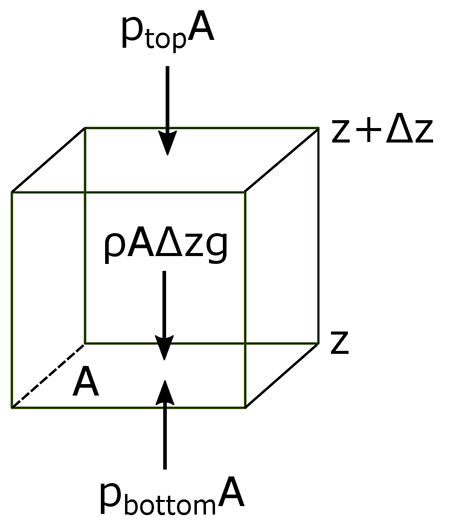
\includegraphics[scale=0.4]{Figuras/L2_hydrostatic_copy.png}
	\caption{Esquema representando las fuerzas en juego en una parcela de un
	fluido en equilibrio hidrostático considerando una forma cúbica de la
	parcela. Haciendo referencia a la ecuación \ref*{balanceFuerzas_basico},
	\(p_{bottom} = p_{inferior}\) y \(p_{top} = p_{superior}\).
	\cite{eqhsPennStateWebsite}}
	\label{balanceFuerzas_imgCubo}
\end{figure}

\subsection{Fluidos no Ideales}
Para que la ecuación \ref{balanceFuerzas_diferencial} pueda ser aplicada a un
problema particular requiere que la densidad \(\rho\) sea constante en el fluido
a lo largo del espacio y del tiempo, es decir requiere que el problema trate de
un \textit{fluido incompresible}. El plasma en el Sol no cumple con este
requisito; la densidad del plasma varía con la altitud en el Sol. La presión y
la temperatura también dependen de la altitud. En estas situaciones se debe
considerar una \textit{ecuación de estado}, la cual acopla estas variables
fluido entre si. La ecuación de gases ideales es un ejemplo de una ecuación de
estado: \(PV = nRT\), la cual incluye la presión y temperatura explícitamente y
la densidad de manera implícita (\(\rho = \frac{n}{V}\)). Sin embargo, esta
ecuación asume que la temperatura es constante con la altitud; para analizar el
equilibrio hidrostático en la superficie del Sol necesitaremos un modelo cuya
temperatura no sea constante en el espacio.

\subsection{Equilibrio Hidrostático Dentro del Sol}

\subsubsection{Modelo Analítico} \label{sec:modeloAnalitico}

Para el problema resuelto en este proyecto consideramos un modelo del Sol en
equilibrio hidrostático. El Sol está compuesto principalmente de hidrógeno
atómico, el cual funciona como el combustible principal para las reacciones
nucleares que ocurren en su núcleo. Estas reacciones generan la presión interna
que balancea el peso gravitacional del mismo Sol debido a su masa. La presión de
un plasma de hidrógeno ionizado se puede modelar usando la ecuación
\ref{ecEstadoPlasmaHidrogeno}. 

\begin{equ}[!ht]
	\begin{equation} \label{ecEstadoPlasmaHidrogeno}
		p(z) = \frac{2 k_B \rho (z) T(z)}{m_p}
	\end{equation}
	\caption{Ecuación de estado dentro del Sol. \(k_B\) es la constante de
	Boltzmann, \(\rho (z)\) es la densidad con respecto a la altitud, \(T(z)\)
	es la temperatura con respecto a la altitud, y \(m_p\) es la masa molecular
	promedio del fluido, que en el caso del Sol la tomamos como la masa del
	hidrógeno atómico. \cite{newtonianCafe}}
\end{equ}

Al integrar la ecuación \ref{balanceFuerzas_diferencial} sustituyendo la
ecuación \ref{ecEstadoPlasmaHidrogeno} como la ecuación de estado obtenemos el
siguiente modelo de la presión solar en la ecuación \ref{ecPresionNoIntegrada}.

\begin{equ}[!ht]
	\begin{equation} \label{ecPresionNoIntegrada}
		p(z) = p(z_0) \exp \left(- \frac{m_p g}{2 k_B} \int_{z_0}^{z} \frac{\mathrm{d} z}{T(z)}\right)
	\end{equation}
	\caption{Presión térmica del gas ionizado en la fotosfera del Sol.
	\(p(z_0)\) es la presión a la altitud de referencia, la cual para este
	problema se toma que \(z_0 = 0 \textrm{ Mm}\), la superficie de la
	fotosfera.}
\end{equ}

Para poder integrar la ecuación \ref{ecPresionNoIntegrada} correctamente se debe
considerar un perfil de temperatura dependiente de la altitud, para la cual se
utiliza la ecuación \ref{ecTemperaturaAnalitica}.

\begin{equ}[!ht]
	\begin{equation} \label{ecTemperaturaAnalitica}
		T(z) = \frac{1}{2} T_{cor} \left(1 + dtc + \left(1 - dtc\right) \tanh \left(\frac{z - z_t}{z_w}\right)\right)
	\end{equation}
	\caption{Perfil de temperatura en la fotosfera solar. Este está definido por
	varios constantes obtenidos del Sol: \(dtc = T_{phot} / T_{cor}\), donde
	\(T_{phot} = 6000 \textrm{ K}\) es la temperatura en la base de la fotosfera
	y \(T_{cor} = 1.2 \times 10^6 \textrm{ K}\) es la temperatura en la corona.
	La región de separación entre la fotosfera y la corona viene representada en
	\(z_t = 2 \textrm{ Mm}\) y \(z_w = 0.2 \textrm{ Mm}\), las cuales
	representan la altitud y el grosor de esta región de transición
	respectivamente. \cite{newtonianCafe}} 
\end{equ}

Dado este perfil de temperatura podemos integrar la ecuación
\ref{ecPresionNoIntegrada} para terminar con la ecuación
\ref{ecPresionIntegralAnalitica} integrada para la presión con respecto a la
altitud. Una vez integrada analíticamente se puede usar para encontrar la
presión en la atmósfera solar a una altitud \(z\); esto nos permitirá encontrar
la densidad del plasma usando la ecuación de estado, modificando la ecuación
\ref{ecEstadoPlasmaHidrogeno} para darnos la densidad del plasma, visto en la
ecuación \ref{ecEstadoDensidadAnalitico}.

\begin{equ}[!ht]
	\begin{equation} \label{ecPresionIntegralAnalitica}
		p(z) = p(z_0) \exp \left(
			- \frac{m_p g}{2 k_B} 
			\left(
				\frac{
					\left(dtc - 1\right) \cdot z_w \cdot
					\ln \left(
						dtc \cdot 
						\exp \left(
							\frac{2 z_t}{z_w} - \frac{2 z}{z_w}
						\right) + 1
					\right) 
				}{
					2 \cdot T_{cor} \cdot dtc
				}
				+ \frac{z}{T_{cor}}
			\right)
		\right)
	\end{equation}
	\caption{Ecuación de presión dependiente de la altitud, integrada usando el perfil de temperatura definido.}
\end{equ}

\begin{equ}[!ht]
	\begin{equation} \label{ecEstadoDensidadAnalitico}
		\rho (z) = \frac{m_p p(z)}{2 k_B T(z)}
	\end{equation}
	\caption{Ecuación de estado del plasma ionizado, presentada de una manera
	que facilita encontrar la densidad del plasma a una altitud \(z\) dado la
	presión y temperatura a esta altitud. \cite{newtonianCafe}}
\end{equ}

\subsubsection{Modelo C7} \label{sec:c7Modelo}
El modelo C7 describe el perfil de temperatura del Sol en su estado inactivo
promedio, enfocado en la cromosfera y la región de transición a la corona.
\cite{c7ModelPaper} Este modelo unidimensional e independiente del tiempo está
basado principalmente en observaciones hechas en el ultravioleta extremo. Este
perfil se puede visualizar en la figura \ref{c7TemperaturaGrafica}.

\begin{figure}[!ht]
	\centering
	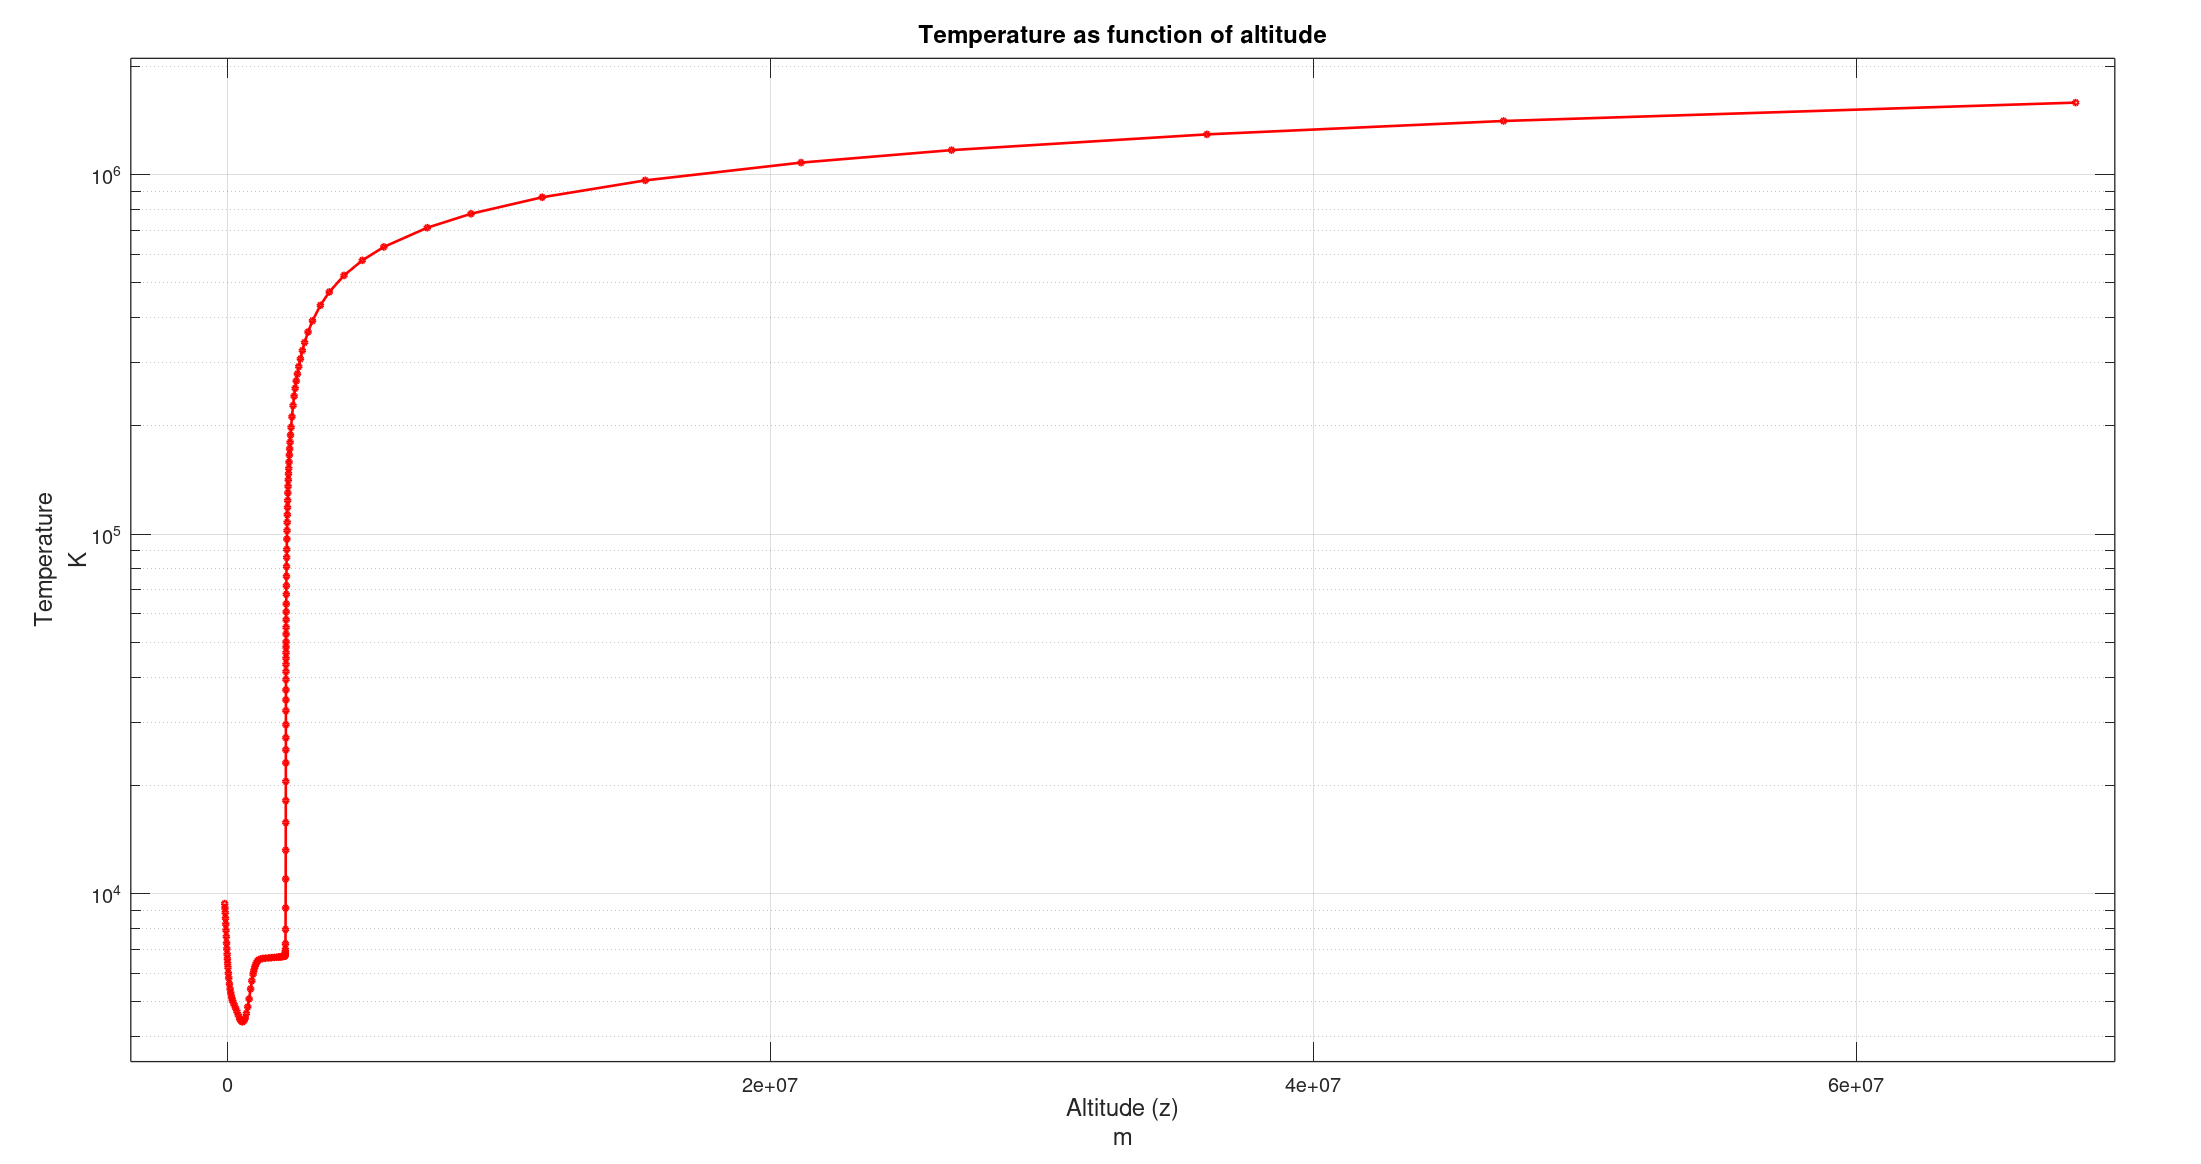
\includegraphics[scale=0.3]{Figuras/C7ModeloTemperaturaGrafica.png}
	\caption{Perfil de temperatura en la cromosfera del Sol, incluyendo la región de transición a la corona. Esta región de transición se puede ver en el fuerte empinamiento de la gráfica, donde la temperatura aumenta rápidamente a niveles mayores de lo visto en la cromosfera.}
	\label{c7TemperaturaGrafica}
\end{figure}

El perfil de temperatura visualizado en la figura \ref{c7TemperaturaGrafica} no
está definido de forma analítica como la ecuación \ref{ecTemperaturaAnalitica},
si no que es un conjunto de datos discretos, dándonos la temperatura en la
atmósfera del Sol a cierta altitud. Para obtener los perfiles de densidad y
presión del plasma en esta región se necesitan las ecuaciones \ref{ecPresionC7}
a \ref{ecScaleHeightC7}:

\begin{equ}[!ht]
	\begin{align}
		p_e (z) = p_{ref} \exp \left(- \int_{z_{ref}}^{z} \frac{dz}{\Lambda (z)}\right) \label{ecPresionC7} \\
		\rho_e (z) = \frac{p_e (z)}{g \Lambda (z)} \label{ecDensidadC7} \\
		\Lambda (z) = \frac{k_B T_e (z)}{m g} \label{ecScaleHeightC7}
	\end{align}
	\caption*{Ecuaciones del equilibrio hidrostático para el modelo C7 de
	temperatura. \cite{newtonianCafe} \(\Lambda (z)\) es la altura de escala, la
	cual modela el decrecimiento de la temperatura del plasma con respecto a la
	altitud.} 
\end{equ}

Debido a la ausencia de una solución analítica para estas ecuaciones, estas
deben ser resueltas usando un método numérico. A continuación explico los
códigos que se desarrollaron para resolver este problema.